\chapter{数学之魅}

% ----------------------------------------------------------------------------------------------------------------------------------------------------------------------
% ----------------------------------------------------------------------------------------------------------------------------------------------------------------------
% ----------------------------------------------------------------------------------------------------------------------------------------------------------------------
\section{求二进制数中1的个数} %%%%%%%%%%%%%%%%%%%%%%%%%%%%%%
\label{sec:number-of-1s-in-binary}


\subsubsection{问题}
对于一个字节(8bit)的无符号整型变量,求其二进制表示中“1”的个数,要求算法的执行效率尽可能高。

\subsubsection{解法一}
利用模运算求取x的每个二进制位上是否为1。
\begin{Codex}[label={[$O(lg(x))+O(1)$]Chap02_01_NumberOfOnes.java}]
int count_1(int x) {
    int ans = 0;
    while (x != 0) {
        ans += (x % 2);
        x /= 2;
    }
    return ans;
}
\end{Codex}

\subsubsection{解法二}
利用位运算求取x的每个二进制位上是否为1。位运算比模运算效率要高。
\begin{Codex}[label={[$O(lg(x))+O(1)$]Chap02_01_NumberOfOnes.java}]
int count_2(int x) {
    int ans = 0;
    while (x != 0) {
        ans += (x & 0x01);
        x >>= 1;
    }
    return ans;
}
\end{Codex}

\subsubsection{解法三}
利用按位与x\&(x-1)每次消除一个1,直到x为0。时间复杂度O(M),,其中M为二进制中1的个数。
\begin{center}
	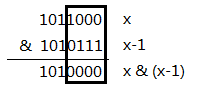
\includegraphics{fig2-1-1.png}\\
	\figcaption{x \& (x-1)}\label{fig:number-of-ones-1}
\end{center}

\begin{Codex}[label={[$O(M)+O(1)$]Chap02_01_NumberOfOnes.java}]
int count_3(int x) {
    int ans = 0;
    while (x != 0) {
        x &= (x - 1);
        ans++;
    }
    return ans;
}
\end{Codex}

\subsubsection{扩展问题1}
如果变量是32位的DWORD,你会使用上述的哪一种算法,或者改进哪一个算法?

\subsubsection{解法}
DWORD是一个32位无符号整数,因此该问题与原问题唯一的区别就是数据的范围不同。上述的三种解法都适用,而且都不要做任何改进。另外对于原书中的解法四使用分支操作和解法五查表法是不适用的。
时间复杂度和空间复杂度和原解法相同。

\subsubsection{扩展问题2}
给定两个正整数(二进制形式表示)A和B,问把A变为B需要改变多少位(bit)?也就是说,整数A和B的二进制表示中有多少位是不同的?

\subsubsection{解法}
拿到这个问题,我们首先想到的就是按照从低到高依次检查A和B的每一位是否相同,然后记录个数,时间复杂度是$O(log_2(Max(A,B)))$。
接着,我们会想能不能把复杂度降到只和位不同的个数相关。自然的就会想到通过一种位运算把不同的1取出来,这种位运算就是按位异或\^{}。计算C=A\^{}B,再计算C中1的个数就行了,可以采用原题中的解法三。


\begin{Codex}[label={[$O(M)+O(1)$]Chap02_01_NumberOfOnes.java}]
int exercise_2(int A, int B) {
    return count(A ^ B);	// 调用上面的count函数,计算A^B中1的个数。
}
\end{Codex}

\subsubsection{扩展问题3}
给定整数$N$,判断它是否为2的幂,比如$0,2,4,8,\cdots$都是2的幂。这是原书中2.2的扩展问题,我感觉放在这里比较合适。

\subsubsection{解法}
\begin{Codex}[label={[$O(1)+O(1)$]Chap02_01_NumberOfOnes.java}]
boolean isPowerOf2(int N) {
    if (N >= 0 && ((N & (N - 1)) == 0)) return true;
    return false;
}
\end{Codex}

% ----------------------------------------------------------------------------------------------------------------------------------------------------------------------
% ----------------------------------------------------------------------------------------------------------------------------------------------------------------------
% ----------------------------------------------------------------------------------------------------------------------------------------------------------------------
\section{不要被阶乘吓倒} %%%%%%%%%%%%%%%%%%%%%%%%%%%%%%
\label{sec:factorial-zeros}

\subsubsection{问题}
1. 给定一个整数$N$,那么$N$的阶乘$N!$末尾有多少个0呢?例如,$N=10$,$N!=3628800$,$N!$的末尾有两个0。

2. 求$N!$的二进制表示中最低位1的位置。

\subsubsection{问题1解法}
对$N!$进行质因数分解得到$N!=\prod {p_i}^{k_i}$,由于10=2×5,所以$N!$末尾0的个数只和5的指数有关。
计算$N!$中有多少个5,可以利用公式$\lfloor\frac{N}{5}\rfloor+\lfloor\frac{N}{5^2}\rfloor+\lfloor\frac{N}{5^3}\rfloor+\cdots$.
\begin{Codex}[label={[$O(log5(N))+O(1)$]Chap02_02_Factorial.java}]
int count_1(int N) {
    int ans = 0;
	while (N != 0) {
        N /= 5;
        ans += N;
    }
    return ans;
}
\end{Codex}

\subsubsection{问题2解法一}
和问题1基本相同,只是现在二进制表示中末尾0的个数是和$N!$中2的指数有关。利用公式$\lfloor\frac{N}{2}\rfloor+\lfloor\frac{N}{2^2}\rfloor+\lfloor\frac{N}{2^3}\rfloor+\cdots$.
\begin{Codex}[label={[$O(lg(N))+O(1)$]Chap02_02_Factorial.java}]
int count_base_2(int N) {
    int ans = 0;
    while (N != 0) {
        N >>= 1;
        ans += N;
    }
    return ans;
}
\end{Codex}

\subsubsection{问题2解法二}
$N!$中质因数2的个数等于$N-N$的二进制表示中1的个数。时间复杂度O(M),M是$N$二进制表示中1的个数。这个解法技巧性太强了,不看解答完全想不到,而且扩展性差。

代码略。

\subsubsection{扩展问题}
求整数N的B进制表示中末尾0的个数。题目来源UVA 10061.

\subsubsection{解法}
对$N!$进行质因数分解得到$N!=\prod {p_i}^{k_i}$,对B进行质因数分解得到$N!=\prod {p_i}^{t_i}$,我们用$f(N,B)$来表示N的B进制表示中末尾0的个数,可以得出下面的等式:
$f(N,B) = min\{\frac{k_i}{t_i}\}$.
\begin{Codex}[label={[$O(lgB(N))+O(1)$]Chap02_02_Factorial.java}]
int countZeros(int n, int b) {
    int ans = Integer.MAX_VALUE;
    for (int i = 2; i <= b; i++) {
        if (b % i != 0) continue;
        int cnt = 0;
        while (b % i == 0) {
            b /= i;
            cnt++;
        }
        int tmp = 0, tn = n;
        while (tn != 0) {
            tn /= i;
            tmp += tn;
        }
        ans = Math.min(ans, tmp / cnt);
    }
    return ans;
}
\end{Codex}
这里我们可以考虑一个问题,可不可以直接求出最大的${p_i}^{t_i}$,然后计算$N!$中有多少个${p_i}$。提示:N=4,B=40.

\section{寻找发帖“水王”} %%%%%%%%%%%%%%%%%%%%%%%%%%%%%%
\label{sec:water-king}

% ----------------------------------------------------------------------------------------------------------------------------------------------------------------------
% ----------------------------------------------------------------------------------------------------------------------------------------------------------------------
% ----------------------------------------------------------------------------------------------------------------------------------------------------------------------
\subsubsection{问题}
给定一个整型数组,每个数组元素表示一个ID,数组长度为N,数组中有一个ID出现的次数超过了数组长度的一半,求出这个ID。

\subsubsection{解法1}
最简单的解法就是暴力枚举每一个数组元素,判断该元素是否超过一半。时间复杂度是$O(N^2)$。

然后我们考虑对数组进行排序(很多问题一旦排序之后就会有思路了),这时候数组的中位数一定就是我们要求的ID。时间复杂度是$O(Nlg(N))$。

最后,我们考虑这样一个场景,让不同的ID进行PK,最后剩下的一定就是超过一半的ID。可以用一个栈来模拟数组中的元素PK的过程。

\begin{Codex}[label={[$O(N)+O(N)$]Chap02_03_WaterKing.java}]
int findMostWithStack(int[] ids) {
    Stack<Integer> stack = new Stack<Integer>();
    for(int i=0;i<ids.length;i++) {
        if(stack.isEmpty()) {
            stack.push(ids[i]);
        } else {
            if(stack.peek()==ids[i]) stack.push(ids[i]);
            else stack.pop();
        }
    }
    return stack.peek();
}
\end{Codex}

\subsubsection{解法2}
下面我们就来考虑一下是否可以降低空间复杂度。其实上面的做法中我们对于栈中的元素并不关心,我们只关心当前栈顶元素和栈的大小,所以我们就可以不用栈来处理了,用两个变量记录栈的大小和栈顶元素即可。

\begin{Codex}[label={[$O(N)+O(1)$]Chap02_03_WaterKing.java}]
int findMost(int[] ids) {
    int candidate = -1, count = 0;
    for (int i = 0; i < ids.length; i++) {
        if (count == 0) {
            candidate = ids[i];
            count = 1;
        } else {
            if (ids[i] == candidate) count++;
            else count--;
        }
    }
    return candidate;
}
\end{Codex}

\subsubsection{解法3}
利用哈希表。


\subsubsection{扩展问题1}
原问题中保证一定存在一个元素超过一半,那么如果去掉这个条件呢?求出这个元素的下标(数组下标从0开始),如果不存在则返回-1.

\subsubsection{解法}
如果不存在超过一半的元素,上面的两个解法其实并不能正确返回。比如[1,2,3],返回的就是3.其实这里要做的就是对这个得到的结果进行判断出现次数是否超过一半,时间和空间复杂度都不改变。

代码略。
\subsubsection{扩展问题2}
有3个元素出现的次数超过了数组长度的$\frac{1}{4}$,找出这3个元素。

\subsubsection{解法}
先排序再查找是可以找出的,时间复杂度是$O(Nlg(N))$,这里就不给出具体代码了。我们同样也可以采用PK的方式来决出次数最多的3个数字,这样就需要保存3个候选元素和它们对应的次数,在遇到新的元素时,先跟这个3个候选元素比较,
如果次数为0就把当前元素作为候选元素,如果当前元素与候选元素相等那么把它的次数加1,如果当前元素与3个候选元素都不相等就把3个候选元素的次数都减去1,最后得到的3个候选元素就是答案了。

我们还可以将问题抽象成一个通用的情况:有k-1个元素出现了超过$\frac{1}{k}$次,求出这k-1个元素。

\begin{Codex}[label={[$O(N)+O(1)$]Chap02_03_WaterKing.java}]
int[] majorityNumber(ArrayList<Integer> nums, int k) {
    int[] candidates = new int[k];
    int[] count = new int[k];
    for (int i = 0; i < nums.size(); i++) {
        int cur = nums.get(i), j;
        for (j = 0; j < k; j++) {
            if (count[j] == 0) {
                candidates[j] = cur;
                count[j]++;
                break;
            } else if (candidates[j] == cur) {
                count[j]++;
                break;
            }
        }
        if (j >= k) {
            for(int idx=0;idx<k;idx++) {
                count[idx]--;
            }
        }
    }
    return candidates;
}
\end{Codex}


% ----------------------------------------------------------------------------------------------------------------------------------------------------------------------
% ----------------------------------------------------------------------------------------------------------------------------------------------------------------------
% ----------------------------------------------------------------------------------------------------------------------------------------------------------------------
\section{1的数目} %%%%%%%%%%%%%%%%%%%%%%%%%%%%%%
\label{sec:number-of-ones-in-sequence}

\subsubsection{问题}
从1到N,顺序写下这N个数字,比如1,2,3,4,...,数一下这其中出现了多少次数字"1"。

1. 定义函数$f(N)$返回1到N之间出现的1的个数,比如$f(12)=5$。

2.满足条件$f(N) = N$ 的最大的N是多少?

\subsubsection{问题1解法}
如果从1到N遍历每一个数字并且求出每个数字中包含了几个1,这种做法的时间复杂度是$O(N*log_{10}(N))$。

我们可以这样考虑,我们首先观察个位数字是循环出现的,循环节是10,每10个数字出现一个1.
\[\underbrace {0, \underline{1}, 2 \cdots , 8, 9}_{10}\]
再来观察一下十位数,这次每100个数字就会出现10个1.
\[\underbrace {0, 1, 2 \cdots , 8, 9, \underline{1}0, \underline{1}1, \underline{1}2, \underline{1}3, \underline{1}4, \underline{1}5, \underline{1}6, \underline{1}7, \underline{1}8, \underline{1}9, 20, 21, \cdots , 98, 99}_{100}\]
同理,百位上每1000个数字出现100个1 $\cdots$

下面,我们举个例子说明一下怎么求1出现的次数。N=1231,先看个位,总共会循环123+1次,每个循环有1个1,再看十位,总共循环12+1次,每个循环有10个1,再看百位,总共循环1+1次,每个循环有100个1,最后是千位,总共循环0.232次,每个循环有1000个1.

关键问题就是如何求循环次数,我们考虑第K位(个位是第0位),digit为当前位上的数字,higher为高位的数字,lower为低位的数字。digit和1的关系有三种:

1. digit=0,循环次数为higher,出现次数为$higher*10^K$。

2. digit=1,循环次数为higher,出现次数为$higher*10^K+lower+1$。

3. digit>1,循环次数为higher+1,出现次数为$(higher+1)*10^K$。


\begin{Codex}[label={[$O(log10(N))+O(1)$]Chap02_04_Ones.java}]
int digitCounts(int n) {
    int ans = 0;
    int power = 1;
    int higher = 0, lower = 0;
    while (n != 0) {
        int digit = n % 10;
        higher = n / 10;
        ans += (higher + (digit > 1 ? 1 : 0)) * power;
        if (digit == 1) {
            ans += lower + 1;
        }
        lower += power * digit;
        power *= 10;
        n /= 10;
    }
    return ans;
}
\end{Codex}

\subsubsection{问题2解法}
无

\subsubsection{扩展问题1}
现在给你你一个数字$K, K \in [0, 1, 2, \cdots , 8, 9]$。求1到N中出现K的次数。题目来源 Lint Code Digit Count。

\subsubsection{解法}
和原问题基本一致,只不过要特殊考虑一下0,因为0不能作为数字开头。

\subsubsection{扩展问题2}
对于其他进制表示方法,也可以试试,看看什么规律。例如二进制:

$f(1) = 1$

$f(10) = 10$ (01,10两个1)

$f(11) = 100$ (01, 10, 11四个1)


\subsubsection{解法}
和十进制的做法基本一致,为了方便计算我们采用十进制来表示数字,比如上面第三个式子我们用十进制表示为$f(3) = 4$,也就是输入输出都是十进制数,但是计算1的个数是采用二进制数。这里给出的代码采用的很多位运算。
\begin{Codex}[label={[$O(lg(N))+O(1)$]Chap02_04_Ones.java}]
int digitCountsBinary(int n) {
    int ans = 0;
    int wei = 0;
    int higher = 0, lower = 0;
    while (n != 0) {
        int digit = n & 0x01;
        higher = n >> 1;
        if (digit == 0) {
            ans += (higher << wei);
        } else {
        ans += ((higher << wei) | lower) + 1;
        }
        lower += (digit << wei);
        wei++;
        n >>= 1;
    }
    return ans;
}
\end{Codex}

% ----------------------------------------------------------------------------------------------------------------------------------------------------------------------
% ----------------------------------------------------------------------------------------------------------------------------------------------------------------------
% ----------------------------------------------------------------------------------------------------------------------------------------------------------------------
\section{寻找最大的K个数} %%%%%%%%%%%%%%%%%%%%%%%%%%%%%%
\label{sec:find-k-great-number}

\subsubsection{问题}
给你个很大的数组,求出这个数组最大的前K个数。

\subsubsection{解法}
拿到问题看到前K个,首先就想到了二叉堆,我们维护一个小根堆的二叉堆,用来保存最大的K个数。然后不断的遍历数组,每遇到一个新的元素就让它进堆,如果堆的大小大于K了,就把最小的元素删除,继续保持小根堆的性质不变。
这样做既可以处理很大的数组,而且可以处理动态到来的元素,是一个在线算法。维护一个二叉堆的时间复杂度是$O(lg(K))$,总的复杂度是$O(N*lg(K))$,N为数组长度。我们在具体的实现的时候,可以直接用PriorityQueue类来维护二叉堆。
\begin{Codex}[label={[$O(N*lg(K))+O(K)$]Chap02_05_FindKthNumber.java}]
int[] findMostKthNumber(int[] nums, int k) {
    PriorityQueue<Integer> queue = new PriorityQueue<Integer>(k + 1);
    for (int num : nums) {
        queue.offer(num);
        if (queue.size() > k) {
            queue.poll();
        }
    }
    int[] ans = new int[k];
    for (int i = 0; i < k; i++) {
        ans[i] = queue.poll();
    }
    return ans;
}
\end{Codex}


% ----------------------------------------------------------------------------------------------------------------------------------------------------------------------
% ----------------------------------------------------------------------------------------------------------------------------------------------------------------------
% ----------------------------------------------------------------------------------------------------------------------------------------------------------------------
\section{精确表达浮点数} %%%%%%%%%%%%%%%%%%%%%%%%%%%%%%
\label{sec:float-number}

\subsubsection{问题}
用分数表示小数。
\[ 0.9 = \frac{9}{10} \]
\[ 0.333(3) = \frac{1}{3} \]
\[ 0.1(2) = \frac{11}{90} \]
左边小数中括号部分为循环节。

\subsubsection{解法}

我们用$0.\overbrace{a_1 \cdots a_k}^{k} \overbrace{(b_1 \cdots b_c)}^{c}$表示小数,其中非循环节部分长度为$k$,数值表示为$\overline{a_1 \cdots a_k}$,循环节部分长度为$c$,数值表示为$\overline{b_1 \cdots b_c}$。我们将最终要求的分数表示成$\frac{A}{B}$

下面我们用公式推导出A和B。
\[ x = 0.\overbrace{a_1 \cdots a_k}^{k} \overbrace{(b_1 \cdots b_c)}^{c}  \]
\[ 10^k*x = \overline{a_1 \cdots a_k}.(\overline{b_1 \cdots b_c}) \]
\[ 10^{k+c}*x = \overline{a_1 \cdots a_kb_1 \cdots b_c}.(\overline{b_1 \cdots b_c}) \]
\[ (10^{k+c}-10^{k}) * x = \overline{a_1 \cdots a_kb_1 \cdots b_c}-\overline{a_1 \cdots a_k} \]
\[ x = \frac{A}{B} = \frac{\overline{a_1 \cdots a_kb_1 \cdots b_c}-\overline{a_1 \cdots a_k}}{10^k*(10^c-1)} = \frac{\overline{a_1 \cdots a_k}*(10^c-1) + \overline{b_1 \cdots b_c}}{10^k*(10^c-1)} \]
\[ A = \overline{a_1 \cdots a_k}*(10^c-1) + \overline{b_1 \cdots b_c} \]
\[ B = 10^k*(10^c-1) \]
\begin{Codex}[label={[$O(N)+O(1)$]Chap02_06_FloatNumber.java}]
int[] floatNubmer(String number) {
    int[] fraction = new int[2];
    int pre = 0, cycle = 0;
    int powerPre =1, powerCycle=1;
    boolean flag = false;
    for(int i=2;i<number.length() && number.charAt(i)!=')';i++) {
        if(number.charAt(i)=='(') {
            flag = true;
            continue;
        }
        if(flag) {
            cycle = cycle * 10 + number.charAt(i)-'0';
            powerCycle*=10;
         } else {
            pre = pre * 10 + number.charAt(i) - '0';
            powerPre*=10;
        }
    }
    if(flag) {
        fraction[0] = pre * (powerCycle - 1) + cycle;
        fraction[1] = powerPre * (powerCycle - 1);
    } else {
        fraction[0] = pre;
        fraction[1] = powerPre;
    }
    int d = gcd(fraction[0], fraction[1]);
    fraction[0] /= d;
    fraction[1] /= d;
    return fraction;
}

int gcd(int a, int b) {
    if(a==0) return b;
    return gcd(b%a, a);
}
\end{Codex}

% ----------------------------------------------------------------------------------------------------------------------------------------------------------------------
% ----------------------------------------------------------------------------------------------------------------------------------------------------------------------
% ----------------------------------------------------------------------------------------------------------------------------------------------------------------------
\section{最大公约数问题} %%%%%%%%%%%%%%%%%%%%%%%%%%%%%%
\label{sec:gcd}

\subsubsection{问题}
求两个正整数的最大公约数(GCD),如果两个正整数很大,有简单的算法吗?

\subsubsection{解法1}

根据欧几里德的辗转相除法可知$gcd(x, y) = gcd(y, x \% y)$。因此可以采用简单的递归来求解最大公约数。

\begin{Codex}[label={[$O(lg(Max(x,y)))+O(1)$]Chap02_07_GCD.java}]
int gcd(int x, int y) {
	if(x==0) return y;
	return gcd(y, x % y);
}
// 非递归形式
int gcd(int x, int y) {
	while(y != 0) {
		int r = x % y;
		m = n;
		n = r;
	}
	return x;
}
\end{Codex}

\subsubsection{解法2}

当正整数很大的时候,取模运算的开销很大,因此要避免使用取模运算。下面给出一种利用奇偶性来计算最大公约数的方法。
\begin{enumerate}
	\item 当x, y均为偶数时,$gcd(x,y) = 2 * gcd(\frac{x}{2}, \frac{y}{2})$。	
	\item 当x, y均为奇数时,$gcd(x,y) = 2 * gcd(y, x-y)$。
	\item 当x为偶数,y为奇数时,$gcd(x,y) = gcd(\frac{y}{2}, y)$。
	\item 当x为奇数,y为偶数时,$gcd(x,y) = gcd(x, \frac{y}{2})$。
\end{enumerate}

\begin{Codex}[label={[$O(lg(Max(x,y)))+O(1)$]Chap02_07_GCD.java}]
BigInteger gcd(BigInteger x, BigInteger y) {
    if (x.compareTo(y) < 0) {
        return gcd(y, x);
    }
    if (y.equals(BigInteger.ZERO)) {
        return x;
    }
    if (isEven(x)) {
        if (isEven(y)) { // x is even, y is even
    	    return gcd(x.divide(BIG_TWO), y.divide(BIG_TWO)).multiply(BIG_TWO);
        } else { // x is even, y is odd
            return gcd(x.divide(BIG_TWO), y);	
        }
    } else {
        if (isEven(y)) { // x is odd, y is even
            return gcd(x, y.divide(BIG_TWO));
        } else { // x is odd, y is odd
            return gcd(y, x.subtract(y));
        }
    }
}

public boolean isEven(BigInteger x) {
	return x.mod(BIG_TWO).equals(BigInteger.ZERO);
}
\end{Codex}

% ----------------------------------------------------------------------------------------------------------------------------------------------------------------------
% ----------------------------------------------------------------------------------------------------------------------------------------------------------------------
% ----------------------------------------------------------------------------------------------------------------------------------------------------------------------
\section{找符合条件的整数} %%%%%%%%%%%%%%%%%%%%%%%%%%%%%%
\label{sec:find-number}

\subsubsection{问题}
任意给定一个正整数N,求一个最小的正整数M(M>1),使得N×M的十进制表示形式里只含有0,1.


% ----------------------------------------------------------------------------------------------------------------------------------------------------------------------
% ----------------------------------------------------------------------------------------------------------------------------------------------------------------------
% ----------------------------------------------------------------------------------------------------------------------------------------------------------------------
\section{斐波纳契数列} %%%%%%%%%%%%%%%%%%%%%%%%%%%%%%
\label{sec:fibonacci}

\subsubsection{问题}
斐波纳契数列的递推公式为:
\[
F(n) = 
\left\{
	\begin{array}{lll}
	0 & \mbox{if} & n=0; \\
	1 & \mbox{if} & n=1; \\
	F(n-1) + F(n-2) & \mbox{if} & n>1.
	\end{array}
\right.
\]
求$F(n)$。
\subsubsection{解法1}
记录每一个计算过的$F(n)$。

\begin{Codex}[label={[$O(N)+O(N)$]Chap02_09_Fibonacci.java}]
int fib(int n) {
    int[] f = new int[n + 1];
    f[0] = 0;
    f[1] = 1;
    for (int i = 2; i <= n; i++) {
    	f[i] = f[i - 1] + f[i - 2];
    }
    return f[n];
}
\end{Codex}

\subsubsection{解法2}
利用特征公式$x^2-x-1=0$求出通向公式为\[F(n)=\frac{1}{\sqrt{5}}×\left[(\frac{1+\sqrt{5}}{2})^n-(\frac{1-\sqrt{5}}{2})^n\right]\]
不过因为引入了无理数,所以不能保证结果的精度。

\begin{Codex}[label={[$O(1)+O(N)$]Chap02_09_Fibonacci.java}]
int fib(int n) {
    double root = Math.sqrt(5.0);
    double ans = (Math.pow((1.0 + root) / 2.0, n) 
    			- Math.pow((1.0 - root) / 2.0, n))
    	 		/ root;
    return (int) ans;
}
\end{Codex}

\subsubsection{解法3}
根据公式
\[
\left[
\begin{array}{cc}
F(n) & F(n-1) \\
F(n-1) & F(n-2) \\
\end{array}
\right]
=
\left[
\begin{array}{cc}
1 & 1 \\
1 & 0 \\
\end{array}
\right]^n
\]

\begin{Codex}[label={[$O(lg(n))+O(N)$]Chap02_09_Fibonacci.java}]
int fib(int n) {
    int[] power = new int[]{1, 1, 1, 0};
    int[] fn = new int[]{1, 0, 1, 0};
    while (n != 0) {
    	if (n % 2 != 0) {
    	    fn = multify(fn, power);
        }
        power = multify(power, power);
        n /= 2;
    }
    return fn[1];
}
int[] multify(int[] x, int[] y) {
    int[] ans = new int[4];
    ans[0] = x[0] * y[0] + x[1] * y[2];
    ans[1] = x[0] * y[1] + x[1] * y[3];
    ans[2] = x[2] * y[0] + x[3] * y[2];
    ans[3] = x[2] * y[1] + x[3] * y[3];
    return ans;
\end{Codex}

% ----------------------------------------------------------------------------------------------------------------------------------------------------------------------
% ----------------------------------------------------------------------------------------------------------------------------------------------------------------------
% ----------------------------------------------------------------------------------------------------------------------------------------------------------------------
\section{寻找数组中的最大值和最小值} %%%%%%%%%%%%%%%%%%%%%%%%%%%%%%
\label{sec:find-maxmin}

\subsubsection{问题}
在数组中找出最大值和最小值,最少需要比较多少次。

\subsubsection{解法1}
扫描一遍数组,将每个数都和最大值最小值比较,需要$2*N$次比较。代码略。

\subsubsection{解法2}
我们每次处理两个数,先比较这两个数,找出比较大的数和最大值比较,找出比较小的数和最小值比较,处理2个数要比较3次,总共需要比较$\frac{3}{2}N$次。

\begin{Codex}[label={[$O(n)+O(1)$]Chap02_10_FindMaxMin.java}]
int[] findMaxMin(int[] nums) {
    int[] maxmin = new int[]{Integer.MIN_VALUE, Integer.MAX_VALUE};
    if (nums.length % 2 != 0) {
        maxmin[0] = maxmin[1] = nums[0];
    }
    for (int i = nums.length % 2; i < nums.length; i += 2) {
    int twoMax = nums[i];
    int twoMin = nums[i + 1];
    if (twoMax < twoMin) {
        twoMax = nums[i + 1];
        twoMin = nums[i];
    }
    maxmin[0] = Math.max(maxmin[0], twoMax);
    maxmin[1] = Math.min(maxmin[1], twoMin);
    }
    return maxmin;
}
\end{Codex}

\subsubsection{扩展问题}
如果需要找出数组中的次大元素,需要比较多少次?

\subsubsection{解法}
和找出最大最小值一样,同时记录最大值和次大值,每次处理两个元素,如果较大的数比最大值大,就更新最大值和次大值,再把较小的数和次大值比较。否则,就把较大的值和次大值比较。比较次数为$\frac{3}{2}N$。

\begin{Codex}[label={[$O(n)+O(1)$]Chap02_10_FindMaxMin.java}]
int findSecondMax(int[] nums) {
    int[] max = new int[]{Integer.MIN_VALUE, Integer.MIN_VALUE};
    if (nums.length % 2 != 0) {
        max[0] = max[1] = nums[0];
    }
    for (int i = nums.length % 2; i < nums.length; i += 2) {
        int mmax = nums[i];
        int smax = nums[i + 1];
        if (mmax < smax) {
            mmax = nums[i + 1];
            smax = nums[i];
        }
        if (mmax > max[0]) {
            max[1] = max[0];
            max[0] = mmax;
            if (smax > max[1]) {
                max[1] = smax;
            }
        } else {
            if (mmax > max[1]) {
                max[1] = mmax;
            }
        }
    }
    return max[1];
}
\end{Codex}


% ----------------------------------------------------------------------------------------------------------------------------------------------------------------------
% ----------------------------------------------------------------------------------------------------------------------------------------------------------------------
% ----------------------------------------------------------------------------------------------------------------------------------------------------------------------
\section{寻找最近点对} %%%%%%%%%%%%%%%%%%%%%%%%%%%%%%
\label{sec:closest-pair-of-points}

\subsubsection{问题}
给定平面上N个点的坐标,找出距离最近的两个点。

\subsubsection{解法}
最直接的方法就是求出每两个点之间的距离,然后找出最小值,这种做法的时间复杂度是$O(n^2)$。我们可以采用分治的方法将时间复杂度降到$O(nlg(n))$。

根据X坐标将这些点从小到大排序,然后分成左右两个部分$S_1$和$S_2$,分别求出它们的最小距离$\delta_1$和$\delta_2$,那么最小距离有三种情况:
\begin{enumerate}
	\item 最近点对都来自$S_1$,那么最小距离为$\delta_1$。
	\item 最近点对都来自$S_2$,那么最小距离为$\delta_2$。
	\item 最近点对分别来自$S_1$和$S_2$,这种情况需要特殊讨论。
\end{enumerate}
下面我们来讨论第三种情况,
\begin{center}
	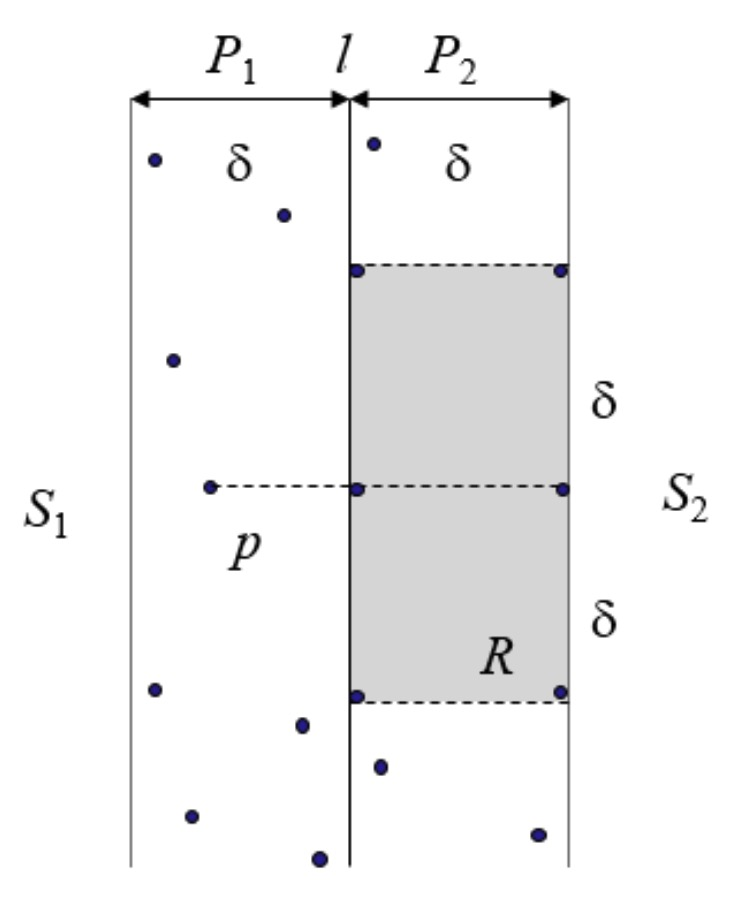
\includegraphics{fig2-11-1.png}\\
	\figcaption{最近点对的三种情况}\label{fig:closest-pair-of-points-1}
\end{center}
如果其中一个点$p$来自$S_1$,另一个点来自$S_2$,那么最多只有6个点和$p$的距离小于$\delta = min(\delta_1, \delta_2)$。如下图所示:
\begin{center}
	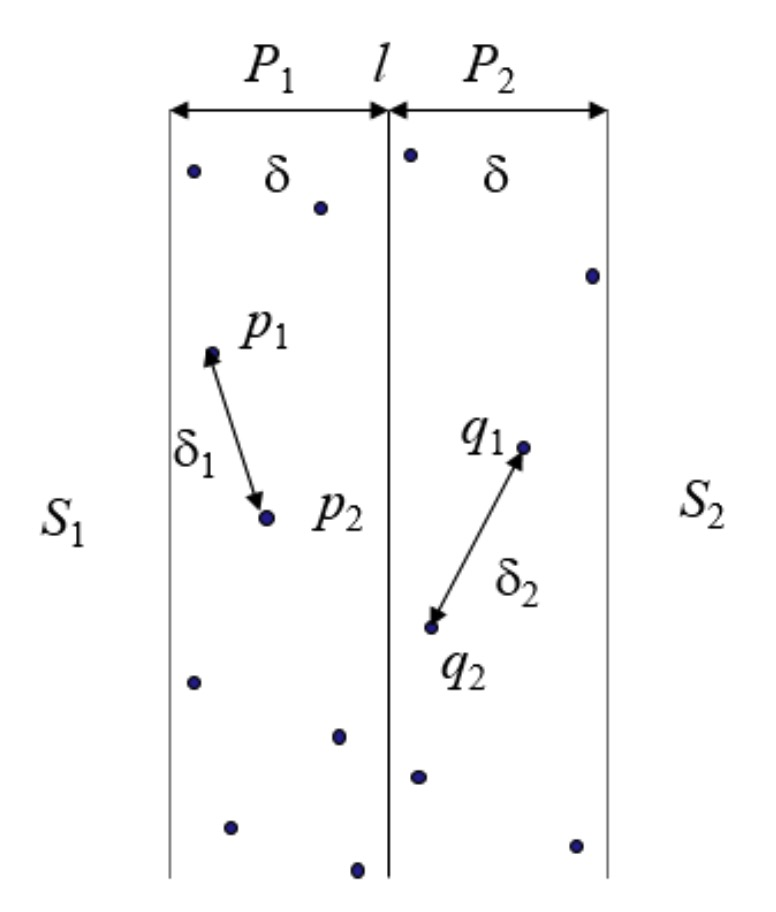
\includegraphics{fig2-11-2.png}\\
	\figcaption{最小距离的区域}\label{fig:closest-pair-of-points-2}
\end{center}
因此我们可以通过对$\delta$范围内的点按照Y坐标排序,这样就能在$O(n)$的时间内求出最小点对。根据时间复杂度$f(n)=2*f(\frac{n}{2})+O(n)$可以求出$f(n)=nlg(n)$。

\begin{Codex}[label={[$O(nlgn)+O(n)$]Chap02_11_ClosestPairOfPoints.java}]
// Point2D的定义
class Point2D {
    int x, y;
    public Point2D(int x, int y) {
        this.x = x;
        this.y = y;
    }
}
double minDist(Point2D[] points) {
	// sort by x
    Arrays.sort(points, new Comparator<Point2D>() {
        @Override
        public int compare(Point2D p, Point2D q) {
            return p.x > q.x ? 1 : -1;
        }
    });
    Point2D[] pointsByY = new Point2D[points.length];
    for (int i = 0; i < points.length; i++) {
        pointsByY[i] = points[i];
    }
	
    Point2D[] aux = new Point2D[points.length];
	
    return closest(points, pointsByY, aux, 0, points.length - 1);
}

private double closest(Point2D[] pointsByX, Point2D[] pointsByY, Point2D[] aux, int start, int end) {
    if (end <= start) {
        return Double.POSITIVE_INFINITY;
    }
	
    int mid = start + (end - start) / 2;
    int median = pointsByX[mid].x;
    double dLeft = closest(pointsByX, pointsByY, aux, start, mid);
    double dRight = closest(pointsByX, pointsByY, aux, mid + 1, end);
    double delta = Math.min(dLeft, dRight);
	
    // O(n)
    merge(pointsByY, aux, start, mid, end);
	
    int count = 0;
    for (int i = start; i <= end; i++) {
        if (Math.abs(pointsByY[i].x - median) < delta) {
            aux[count++] = pointsByY[i];
        }
    }
    // O(n)
    for (int i = 0; i < count; i++) {
        for (int j = i + 1; j < count && aux[j].y - aux[i].y < delta; j++) {
            double distance = dist(aux[i], aux[j]);
            delta = Math.min(delta, distance);
        }
    }
    return delta;
}

private double dist(Point2D p, Point2D q) {
    double dx = p.x - q.x;
    double dy = p.y - q.y;
    return Math.sqrt(dx * dx + dy * dy);
}

private void merge(Point2D[] pointsByY, Point2D[] aux, int start, int mid, int end) {
    for (int i = start; i <= end; i++) {
	    aux[i] = pointsByY[i];
    }
    int i = start, j = mid + 1, k = start;
    while (i <= mid || j <= end) {
        if (j > end || (i <= mid && aux[i].y < aux[j].y)) {
            pointsByY[k++] = aux[i++];
        } else {
            pointsByY[k++] = aux[j++];
        }
    }
}
\end{Codex}

% ----------------------------------------------------------------------------------------------------------------------------------------------------------------------
% ----------------------------------------------------------------------------------------------------------------------------------------------------------------------
% ----------------------------------------------------------------------------------------------------------------------------------------------------------------------
\section{快速寻找满足条件的两个数} %%%%%%%%%%%%%%%%%%%%%%%%%%%%%%
\label{sec:two-sum}

\subsubsection{问题}
快速找出一个数组中的两个数字,使得它们的和等于一个给定的值。

\subsubsection{解法1}
最简单的做法就是穷举:从数组中任意取出两个数字计算它们的和是否为给定的值,时间复杂度为$O(n^2)$。

更快的查找方法是利用哈希表直接查找,将每个数字映射到哈希表中,然后对每个数字在哈希表中查找是否存在另一个数字。时间复杂度是$O(n)$。

\begin{Codex}[label={[$O(n)+O(n)$]Chap02_12_TwoSum.java}]
int[] twoSum(int[] numbers, int target) {
    HashMap<Integer, Integer> map = new HashMap<Integer, Integer>();
    for (int i = 0; i < numbers.length; i++) {
        Integer other = map.get(target - numbers[i]);
        if (other != null) {
            return new int[]{other, i};
        }
        map.put(numbers[i], i);
    }
    return new int[]{-1, -1};
}
\end{Codex}

\subsubsection{解法2}
如果对数组按照从小到大进行排序,那就可以利用二分查找来找出另一个数字是否在数组中,时间复杂度是$O(nlgn)$。另外,我们还可以采用两个指针的想法,让两个指针p,q分别指向数组首部和尾部。如果这两个数的和大于目标值就移动q--,
如果大于目标值就移动p++。

\begin{Codex}[label={[$O(n)+O(1)$]Chap02_12_TwoSum.java}]
// 这里假设数组是升序排列的
int[] twoSum_2(int[] numbers, int target) {
    int i = 0, j = numbers.length - 1;
    while (i < j) {
        if (numbers[i] + numbers[j] > target) {
            j--;
        } else if (numbers[i] + numbers[j] < target) {
            i++;
        } else {
            return new int[]{i, j};
        }
    }
    return new int[]{-1, -1};
}
\end{Codex}

% ----------------------------------------------------------------------------------------------------------------------------------------------------------------------
% ----------------------------------------------------------------------------------------------------------------------------------------------------------------------
% ----------------------------------------------------------------------------------------------------------------------------------------------------------------------
\section{子数组的最大乘积} %%%%%%%%%%%%%%%%%%%%%%%%%%%%%%
\label{sec:max-product}

\subsubsection{问题}
给定一个长度为N的整数数组,只允许使用乘法,不能用除法,计算任意N-1个数的组合中乘积最大的一组。

\subsubsection{解法}
使用两个乘积数组,$left[i]=\prod_{k=0}^{i-1}numbers[k]$,$right[i]=\prod_{k=n-1}^{i+1}numbers[k]$,则$ans = max_{i=0}^{n-1}(left[i]*right[i])$。算法的时间复杂度是O(n)。

\begin{Codex}[label={[$O(n)+O(n)$]Chap02_13_MaxProduct.java}]
int maxProduct(int[] numbers) {
    int len = numbers.length;
    if (len <= 1) {
        return 0;
    }
    int ans = 0;
    int[] leftProduct = new int[len];
    int[] rightProduct = new int[len];
    leftProduct[0] = 1;
    rightProduct[len - 1] = 1;
    for (int i = 1; i < numbers.length; i++) {
        leftProduct[i] = leftProduct[i - 1] * numbers[i - 1];
    }
    for (int i = len - 2; i >= 0; i--) {
        rightProduct[i] = rightProduct[i + 1] * numbers[i + 1];
    }
    for (int i = 0; i < numbers.length; i++) {
        ans = Math.max(ans, leftProduct[i] * rightProduct[i]);
    }
    return ans;
}
\end{Codex}

% ----------------------------------------------------------------------------------------------------------------------------------------------------------------------
% ----------------------------------------------------------------------------------------------------------------------------------------------------------------------
% ----------------------------------------------------------------------------------------------------------------------------------------------------------------------
\section{求数组的子数组之和的最大值} %%%%%%%%%%%%%%%%%%%%%%%%%%%%%%
\label{sec:max-sum}

\subsubsection{问题}
给定一个数组,求出子数组之和的最大值

\subsubsection{解法}

\begin{Codex}[label={[$O(n)+O(1)$]Chap02_14_MaxSubarray.java}]
int maxSubArray(int[] A) {
    int ans = A[0];
    int sum = A[0];
    for (int i = 1; i < A.length; i++) {
        sum = Math.max(A[i], A[i] + sum);
        ans = Math.max(ans, sum);
    }
    return ans;
}
\end{Codex}

% ----------------------------------------------------------------------------------------------------------------------------------------------------------------------
% ----------------------------------------------------------------------------------------------------------------------------------------------------------------------
% ----------------------------------------------------------------------------------------------------------------------------------------------------------------------
\section{子数组之和的最大值(二维)} %%%%%%%%%%%%%%%%%%%%%%%%%%%%%%
\label{sec:max-sum-two-dimon}

\subsubsection{问题}
对于2.14的一维数组可以扩展到二维的数组,如何求出一个矩形区域使得和最大呢?

\subsubsection{解法}
直接将二维投影成一维的情况,然后利用最大子数组的解法求出最大矩形和。算法的时间复杂度是$O(n^2*m)$。

\begin{Codex}[label={[$O(n^2*m)+O(1)$]Chap02_15_MaxSubmatrix.java}]
int maxSubmatrix(int[][] A) {
    int rows = A.length;
    int columns = A[0].length;
    int ans = Integer.MIN_VALUE;
    for (int i = 1; i < rows; i++) {
        for (int j = 0; j < columns; j++) {
            A[i][j] += A[i - 1][j];
        }
    }
    // 枚举起始行和结束行
    for (int i = 0; i < rows; i++) {
        for (int j = i; j < rows; j++) {
            int sum = 0;
            for (int k = 0; k < columns; k++) {
                int x = A[j][k] - (i == 0 ? 0 : A[i - 1][k]);
                sum = Math.max(x, x + sum);
                ans = Math.max(ans, sum);
            }
        }
    }
    return ans;
}
\end{Codex}


% ----------------------------------------------------------------------------------------------------------------------------------------------------------------------
% ----------------------------------------------------------------------------------------------------------------------------------------------------------------------
% ----------------------------------------------------------------------------------------------------------------------------------------------------------------------
\section{求数组中最长递增子序列} %%%%%%%%%%%%%%%%%%%%%%%%%%%%%%
\label{sec:longest-increasing-subsequence}

\subsubsection{问题}
求一个一维数组中最长递增子序列的长度。例如,在序列[1,7,3,6,4,5,2]中,最长递增子序列为[1,3,4,5],长度为4。
\begin{center}
	\Large
	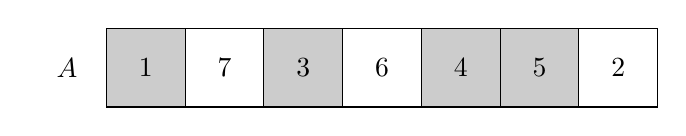
\begin{tikzpicture}[minimum size = 1cm]
		\node at (0,0) [rectangle] {$A$};
		\node at (1,0) [rectangle,draw=black, fill=black!20] {1};
		\node at (2,0) [rectangle,draw] {7};
		\node at (3,0) [rectangle,draw=black, fill=black!20] {3};
		\node at (4,0) [rectangle,draw] {6};
		\node at (5,0) [rectangle,draw=black, fill=black!20] {4};
		\node at (6,0) [rectangle,draw=black, fill=black!20] {5};
		\node at (7,0) [rectangle,draw] {2};
	\end{tikzpicture}
	\figcaption{最长递增子序列}\label{fig:longest-increasing-subsequence-1}
\end{center}

\subsubsection{解法1}
用$f[i]$表示序列$[A_0, A_1, \dots, A_i]$中以$A_i$为结尾的最长递增子序列的长度。利用动态规划,求出状态转移方程为:
\[
f[i] = 
\left\{
\begin{array}{ll}
1 & n=0; \\
max_{A_j<A_i}(f[j]+1) & n>0.
\end{array}
\right.
\]
因此只要遍历每一个元素,计算出$f[i]$并记录$f[i]$的最大值即为最长递增子序列的长度。
\begin{center}
	\Large
	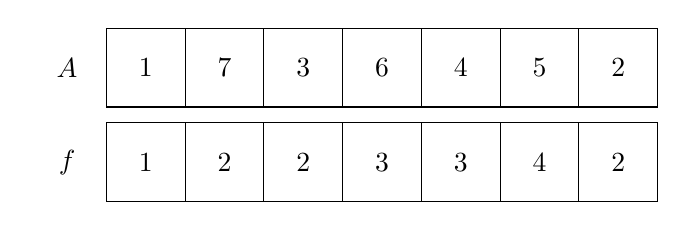
\begin{tikzpicture}[minimum size = 1cm]
	\node at (0,0) [rectangle] {$A$};
	\node at (1,0) [rectangle,draw] {1};
	\node at (2,0) [rectangle,draw] {7};
	\node at (3,0) [rectangle,draw] {3};
	\node at (4,0) [rectangle,draw] {6};
	\node at (5,0) [rectangle,draw] {4};
	\node at (6,0) [rectangle,draw] {5};
	\node at (7,0) [rectangle,draw] {2};
	
	\node at (0,-1.2) [rectangle] {$f$};
	\node at (1,-1.2) [rectangle,draw] {1};
	\node at (2,-1.2) [rectangle,draw] {2};
	\node at (3,-1.2) [rectangle,draw] {2};
	\node at (4,-1.2) [rectangle,draw] {3};
	\node at (5,-1.2) [rectangle,draw] {3};
	\node at (6,-1.2) [rectangle,draw] {4};
	\node at (7,-1.2) [rectangle,draw] {2};
	\end{tikzpicture}
	\figcaption{最长递增子序列求解}\label{fig:longest-increasing-subsequence-2}
\end{center}
\begin{Codex}[label={[$O(n^2)+O(n)$]Chap02_16_LongestIncreasingSubsequence.java}]
int LIS(int[] numbers) {
    int ans = 1;
    int n = numbers.length;
    int[] len = new int[n];
    for (int i = 0; i < n; i++) {
        len[i] = 1;
        for (int j = 0; j < i; j++) {
            if (numbers[i] > numbers[j] && len[j] + 1 > len[i]) {
                len[i] = len[j] + 1;
            }
        }
        ans = Math.max(ans, len[i]);
    }
    return ans;
}
\end{Codex}


% ----------------------------------------------------------------------------------------------------------------------------------------------------------------------
% ----------------------------------------------------------------------------------------------------------------------------------------------------------------------
% ----------------------------------------------------------------------------------------------------------------------------------------------------------------------
\section{数组循环移位} %%%%%%%%%%%%%%%%%%%%%%%%%%%%%%
\label{sec:array-cyclic-shift}

\subsubsection{问题}
把一个含有N个元素的数组循环右移K位,要求时间复杂度为$O(N)$,且只允许使用两个附加变量。

\subsubsection{解法}
比如数组序列为$abcd1234$,要求循环右移4位变成$1234abcd$,我们发现前半段和后半段的相对顺序变了,但是内部顺序没变,因此可以通过整体反转数组然后再局部反转。
\begin{enumerate}
	\item 反转数组,$abcd1234 \Longrightarrow 4321dcba$。
	\item 反转前半部分,$4321dcba \Longrightarrow 1234dcba$。
	\item 反转后半部分,$1234dcba \Longrightarrow 1234abcd$。
\end{enumerate}

\begin{Codex}[label={[$O(n)+O(1)$]Chap02_17_ArrayCyclicShift.java}]
void cyclicShift(int[] numbers, int k) {
    int n = numbers.length;
    k %= n;
    reverse(numbers, 0, n - 1);
    reverse(numbers, 0, n - k - 1);
    reverse(numbers, n - k, n - 1);
}

void reverse(int[] numbers, int start, int end) {
    for (; start < end; start++, end--) {
        int tmp = numbers[start];
        numbers[start] = numbers[end];
        numbers[end] = tmp;
    }
}
\end{Codex}


% ----------------------------------------------------------------------------------------------------------------------------------------------------------------------
% ----------------------------------------------------------------------------------------------------------------------------------------------------------------------
% ----------------------------------------------------------------------------------------------------------------------------------------------------------------------
\section{数组分割} %%%%%%%%%%%%%%%%%%%%%%%%%%%%%%
\label{sec:split-array}

\subsubsection{问题}
有一个无序、元素个数为2n的正整数数组,要求:如何能把这个数组分割为元素个数为n的两个数组,并使两个子数组的和最接近。

\subsubsection{解法}



% ----------------------------------------------------------------------------------------------------------------------------------------------------------------------
% ----------------------------------------------------------------------------------------------------------------------------------------------------------------------
% ----------------------------------------------------------------------------------------------------------------------------------------------------------------------
\section{区间重合判断} %%%%%%%%%%%%%%%%%%%%%%%%%%%%%%
\label{sec:interval-overlapping}

\subsubsection{问题}
给定一个源区间$[x,y](y\geq x)$和N个无序的目标区间$[x_1,y_1][x_2,y_2][x_3,y_3]\dots[x_n,y_n]$,判断源区间$[x,y]$是不是在目标区间内,也即$[x,y]\in \bigcup\limits_{i=1}^{n}[x_i,y_i]$?

\subsubsection{解法}
先将目标区间合并再判断源区间是否在合并之后的目标区间。合并操作可以通过排序进行优化,将目标区间按照x坐标升序排序,然后利用贪心算法从前到后遍历目标区间,如果当前区间和前一个区间有交集,即$x_i<=y_{i-1}$就合并两个区间。
查找源区间是否在目标区间可以词啊用二分查找,只需要查找最后一个x坐标小于源区间x坐标的区间然后判断即可。合并操作需要$O(nlgn)$,查找操作需要O(lgn),总的时间复杂度为$O(nlgn)$。

\begin{Codex}[label={[$O(nlgn)+O(1)$]Chap02_19_IntervalsOverlapping.java}]
class Interval {
	int start, end;
	
	Interval(int s, int e) {
		start = s;
		end = e;
	}
}

boolean isIntervalsOverlapping(Interval[] target, Interval source) {
	if (target.length <= 0) {
		return false;
	}
	int n = merge(target);
	return search(target, source, n);
}

int merge(Interval[] target) {
	Arrays.sort(target, new Comparator<Interval>() {
		@Override
		public int compare(Interval a, Interval b) {
			return a.start > b.start ? 1 : -1;
		}
	});
	int len = 0;
	for (int i = 1; i < target.length; i++) {
		if (target[i].start > target[len].end) {
			target[++len] = target[i];
		} else if (target[i].end > target[len].end) {
		target[len].end = target[i].end;
	}
}
return len + 1;
}

private boolean search(Interval[] target, Interval source, int n) {
	int left = 0, right = n - 1;
	while (left <= right) {
		int mid = left + (right - left) / 2;
		if (source.start >= target[mid].start && source.end <= target[mid].end) {
			return true;
		}
		if (source.start >= target[mid].start) {
			left = mid + 1;
		} else {
		right = mid - 1;
	}
}
return false;
}
\end{Codex}

\subsubsection{扩展问题1}
如何判断两个矩形是否相交?这里给出的矩形的两条边都是平行于坐标轴的。

\subsubsection{解答}
因为这里讨论的矩形都是平行于坐标轴的,所以可以用矩形的左下角和右上角坐标唯一表示一个矩形。
\begin{center}
	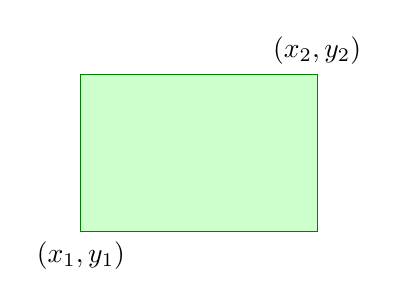
\begin{tikzpicture}
	\filldraw[fill=green!20!white, draw=green!50!black] (1, 1) -- (4, 1) -- (4, 3) -- (1, 3) -- cycle;
	\node at (1, 0.7) [rectangle] {$(x_1,y_1)$};
	\node at (4, 3.3) [rectangle] {$(x_2,y_2)$};
	\end{tikzpicture}
	\figcaption{矩形窗口}\label{fig:rectangle-overlapping-1}
\end{center}

这里先给出矩形的定义:
\begin{Codex}[label={Rectangle.java}]
class Rectangle {
	int x1, y1, x2, y2;
	
	Rectangle(int x1, int y1, int x2, int y2) {
		this.x1 = x1;
		this.y1 = y1;
		this.x2 = x2;
		this.y2 = y2;
	}
}
\end{Codex}

\begin{center}
	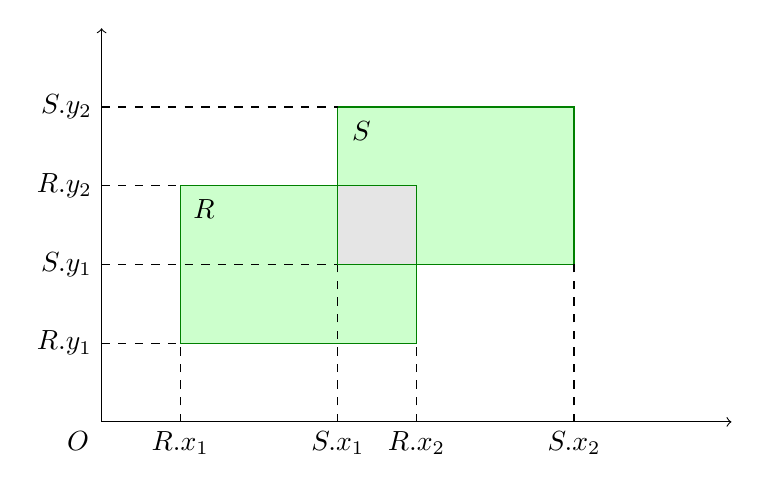
\begin{tikzpicture}
	\draw[->] (0,0) -- (8,0); \draw[->] (0,0) -- (0,5);
	\draw (-0.3,0) node[anchor=north] {$O$};
	\filldraw[fill=green!20!white, draw=green!50!black] (1, 1) -- (4, 1) -- (4, 3) -- (1, 3) -- cycle;
	\draw (1.3,2.7) node {$R$};
	\draw[dashed] (1,0) -- (1,1); \draw[dashed] (4,0) -- (4,1);
	\draw[dashed] (0,1) -- (1,1); \draw[dashed] (0,3) -- (1,3);
	\draw (1,0) node[anchor=north] {$R.x_1$};
	\draw (4,0) node[anchor=north] {$R.x_2$};
	\draw (0,1) node[anchor=east] {$R.y_1$};
	\draw (0,3) node[anchor=east] {$R.y_2$};
		
	\filldraw[fill=green!20!white, draw=green!50!black] (3, 2) -- (6, 2) -- (6, 4) -- (3, 4) -- cycle;
	\draw (3.3,3.7) node {$S$};
	\draw[dashed] (3,0) -- (3,2); \draw[dashed] (6,0) -- (6,2);
	\draw[dashed] (0,2) -- (3,2); \draw[dashed] (0,4) -- (3,4);
	\draw (3,0) node[anchor=north] {$S.x_1$};
	\draw (6,0) node[anchor=north] {$S.x_2$};
	\draw (0,2) node[anchor=east] {$S.y_1$};
	\draw (0,4) node[anchor=east] {$S.y_2$};
	
	\filldraw[fill=gray!20!white, draw=green!50!black] (3, 2) -- (4, 2) -- (4, 3) -- (3, 3) -- cycle;
	\end{tikzpicture}
	\figcaption{矩形窗口相交}\label{fig:rectangle-overlapping-2}
\end{center}
对于平行于坐标轴的两个矩形,我们可以将它们分别投影到X坐标轴和Y坐标轴。矩形R(x1,y1,x2,y2)在X轴上的投影就是线段$[x1,x2]$,在Y轴上的投影就是线段$[y1,y2]$。此时,如果两个矩形在X轴和Y轴上的投影都相交则说明两个矩形相交。
\begin{Codex}[label={[$O(1)+O(1)$]Chap02_19_IntervalsOverlapping.java}]
boolean isRectangleIntersect(Rectangle R, Rectangle S) {
	return R.x1 <= S.x2 && R.x2 >= S.x1 
		&& R.y1 <= S.y2 && R.y2 >= S.y1;
}
\end{Codex}

\subsubsection{扩展问题2}
如何处理二维空间的覆盖问题?例如在Windows桌面上有若干窗口,如何判断某一个窗口是否完全被其他窗口覆盖?

\subsubsection{解答}
\begin{Codex}[label={[$O(n^3)+O(n)$]Chap02_19_IntervalsOverlapping.java}]
private List<Integer> xCoordinate;
private List<Integer> yCoordinate;

boolean isRectangleOverlapping(Rectangle[] rects, Rectangle target) {
	int n = rects.length;
	xCoordinate = new ArrayList<Integer>(2 * (n + 1));
	yCoordinate = new ArrayList<Integer>(2 * (n + 1));
	boolean[][] flag = new boolean[2 * n][2 * n];
	
	for (int i = 0; i < n; i++) {
		addToList(rects[i]);
	}
	addToList(target);
	
	Collections.sort(xCoordinate);
	Collections.sort(yCoordinate);
	
	for (int k = 0; k <= n; k++) {
		Rectangle rect = target;
		if (k < n) {
			rect = rects[k];
		}
		for (int i = 0; i < xCoordinate.size() && xCoordinate.get(i) < rect.x2; i++) {
			if (xCoordinate.get(i) < rect.x1) {
				continue;
			}
			for (int j = 0; j < yCoordinate.size() && yCoordinate.get(j) < rect.y2; j++) {
				if (yCoordinate.get(j) < rect.y1) {
					continue;
				}
				if (k == n && !flag[i][j]) {
					return false;
				}
				flag[i][j] = true;
			}
		}
	}
	return true;
}

private void addToList(Rectangle rect) {
	if (!xCoordinate.contains(rect.x1)) {
		xCoordinate.add(rect.x1);
	}
	if (!xCoordinate.contains(rect.x2)) {
		xCoordinate.add(rect.x2);
	}
	if (!yCoordinate.contains(rect.y1)) {
		yCoordinate.add(rect.y1);
	}
	if (!yCoordinate.contains(rect.y2)) {
		yCoordinate.add(rect.y2);
	}
}
\end{Codex}

% ----------------------------------------------------------------------------------------------------------------------------------------------------------------------
% ----------------------------------------------------------------------------------------------------------------------------------------------------------------------
% ----------------------------------------------------------------------------------------------------------------------------------------------------------------------
\section{程序理解和时间分析} %%%%%%%%%%%%%%%%%%%%%%%%%%%%%%
\label{sec:time-analysis}

\subsubsection{问题}
阅读程序,回答一下问题:
\begin{Codex}[label={Chap02_19_IntervalsOverlapping.java}]
public static void main(String[] args) {
	long startTime = System.currentTimeMillis();
	int[] rg = new int[]{2, 3, 4, 5, 6, 7, 8, 9, 10, 11, 12, 13, 14, 15, 16,
		17, 18, 19, 20, 21, 22, 23, 24, 25, 26, 27, 28, 29, 30, 31};
	for (long i = 1; i < Long.MAX_VALUE; i++) {
		int hit = 0;
		int hit1 = -1;
		int hit2 = -1;
		for (int j = 0; j < rg.length && hit <= 2; j++) {
			if (i % rg[j] != 0) {
				hit++;
				if (hit == 1) {
					hit1 = j;
				} else if (hit == 2) {
					hit2 = j;
				} else {
					break;
				}
			}
		}
		if (hit == 2 && hit1 + 1 == hit2) {
			System.out.println(i);
			break;
		}
	}
	long endTime = System.currentTimeMillis();
	System.out.println(endTime-startTime);
}
\end{Codex}

\begin{enumerate}
	\item 这个程序要找的是符合什么条件的数?
	\item 这样的数存在吗?符合这一条件的最小数是什么?
	\item 在电脑上运行这一程序,你估计多长时间才能输出第一个结果?时间精确到分钟。
\end{enumerate}


\subsubsection{解法}
根据if (hit == 2 \&\& hit1 + 1 == hit2)这一行代码可以看出程序要找的数字$N$满足:
\begin{enumerate}
	\item 在$[2,3,\dots,31]$中,只有两个数$K_1$和$K_2$不能整除$N$。
	\item 而且这两个不能整除$N$的数相差为1,即$K_1+1=K_2$。
\end{enumerate}
我们可以先假设满足条件的$K_1=2,K_2=3$,那么其他整数都能整除$N$,但是很明显只要能被4整除就能被2整除。因此,我们可以想到只有能被16,17整除,但是不被其他整除的数字。所以$N=2^3*3^2*5^2*7*11*13*19*23*29*31=2123581660200$。

% ----------------------------------------------------------------------------------------------------------------------------------------------------------------------
% ----------------------------------------------------------------------------------------------------------------------------------------------------------------------
% ----------------------------------------------------------------------------------------------------------------------------------------------------------------------
\section{只考加法的面试题} %%%%%%%%%%%%%%%%%%%%%%%%%%%%%%
\label{sec:add}

\subsubsection{问题}
一个整数可以表示成一系列连续整数的和,比如$9=4+5=2+3+4$。
\begin{enumerate}
	\item 写一个程序,对于一个64位正整数N,输出N所有可能的连续自然数之和的算式。
	\item 有一些数字不能表示成连续自然数的和,这些数有什么规律,能否证明。
	\item 64位正整数范围内,子序列数目最多的数是哪个数?
\end{enumerate}

\subsubsection{解法}
\begin{Codex}[label={[$O(nlgn)+O(1)$]Chap02_21_Add.java}]
List<List<Long>> output(long number) {
	long left = 1;
	List<List<Long>> ans = new ArrayList<List<Long>>();
	for (long i = 2; i < Math.sqrt(2) * Math.sqrt(number); i++) {
		if ((number - left) % i == 0) {
			List<Long> list = new ArrayList<Long>();
			for (long j = (number - left) / i; j < (number - left) / i + i; j++) {
				list.add(j);
			}
			ans.add(list);
		}
		left += i;
	}
	return ans;
}
\end{Codex}

$2^n(n\geq 0)$不能表示为连续自然数的和。

猜想:N的子序列个数。

子序列数目最多的一个数是$3^4*5^3*7*11*13*17*19*23*29*31*37*41*47$。